% !TEX root = ../main.tex

\chapter{Medical information}
\label{ch:medical}

\section{Cancer}


\subsection{Basics}
An accumulation of cells forming a mass is called a tumor. These tumors are detectable thanks to medical imaging (see section \ref{sec:medical_imaging}) and other symptoms. However, not every tumor is as dangerous as the other, as it can be benign (does not contain cancerous cells) or malignant (contains cancerous cells).

The term cancer refers to different phenomena which involve mutation, abnormal multiplication and spreading of cells. As stated by Hanahan et al. in "The Hallmarks of Cancer" \cite{19} and "The Hallmarks of Cancer: The Next Generation" \cite{20}, every malignant tumor acquires six different capabilities during its evolution: 
\begin{itemize}
	\item \textbf{"Sustaining proliferative signaling"}\\ Cancerous cells don't wait for the body's approval to grow and proliferate, contrary to normal cells. They become the only responsible for their multiplication.
	\item \textbf{"Evading growth suppressors"}\\
The body sends signals to contain cell growth within a tissue. Cancerous cells are insensitive to these. 
	\item \textbf{"Activating invasion and metastasis"}\\
Metastases are cells whose role is to propagate to other parts of the body in order to colonize and create new tumors. 
	\item \textbf{"Enabling replicative immortality"}\\
Healthy cells replication is limited to a certain amount, which is not the case for cancerous cells. 
	\item \textbf{"Inducing angiogenesis"}
\\Angiogenesis is the process of creating new blood vessels. Tumors have an influence on angiogenesis around them, since they need vascularization to continue growing. 
	\item \textbf{"Resisting cell death"}
\\Apoptosis is the programmed death of cells, which is part of the continuous regeneration of every cell within a body. Cancerous cells survive this programmed death. 
	
\end{itemize}


\subsection{Seriousness}

Most cancers can be staged thanks to the TNM system. The T corresponds to the tumor size and its location; the N corresponds to whether or not the tumor has spread to draining lymph nodes; the M corresponds to the presence or absence of metastases in other parts of the body \cite{21}. These pieces of information are used to classify cancer between four (I to IV) or sometimes five (0 to IV) different stages, reflecting the progression and the seriousness of the illness \cite{22}. The earlier they are detected, the higher the chances of recovering are.

%\subsection{Chronological evolution}


\section{Medical imaging}
\label{sec:medical_imaging}

Multiple types of medical imaging exist. The most commonly used to detect cancer are Magnetic Resonance Imaging (MRI), CT (Computed Tomography) scans
%, PET (Positron Emission Tomography) scans
and mammographies. 

MRI relies on magnetic fields to provide a three-dimensional view of body parts, which allows to see the outputed images as a volume. Different settings, usually called sequences, make the look of the output vary, as shown on figure \ref{fig:PROSTATEx-t2-adc-dwi}.
Unlike MRI, CT is based on X-rays instead of magnetic fields, but still provides a three-dimensional representation of a body part. Figure \ref{fig:visualize_lung_dcm} shows a lung CT scan.

\begin{figure}[!h]
\centering
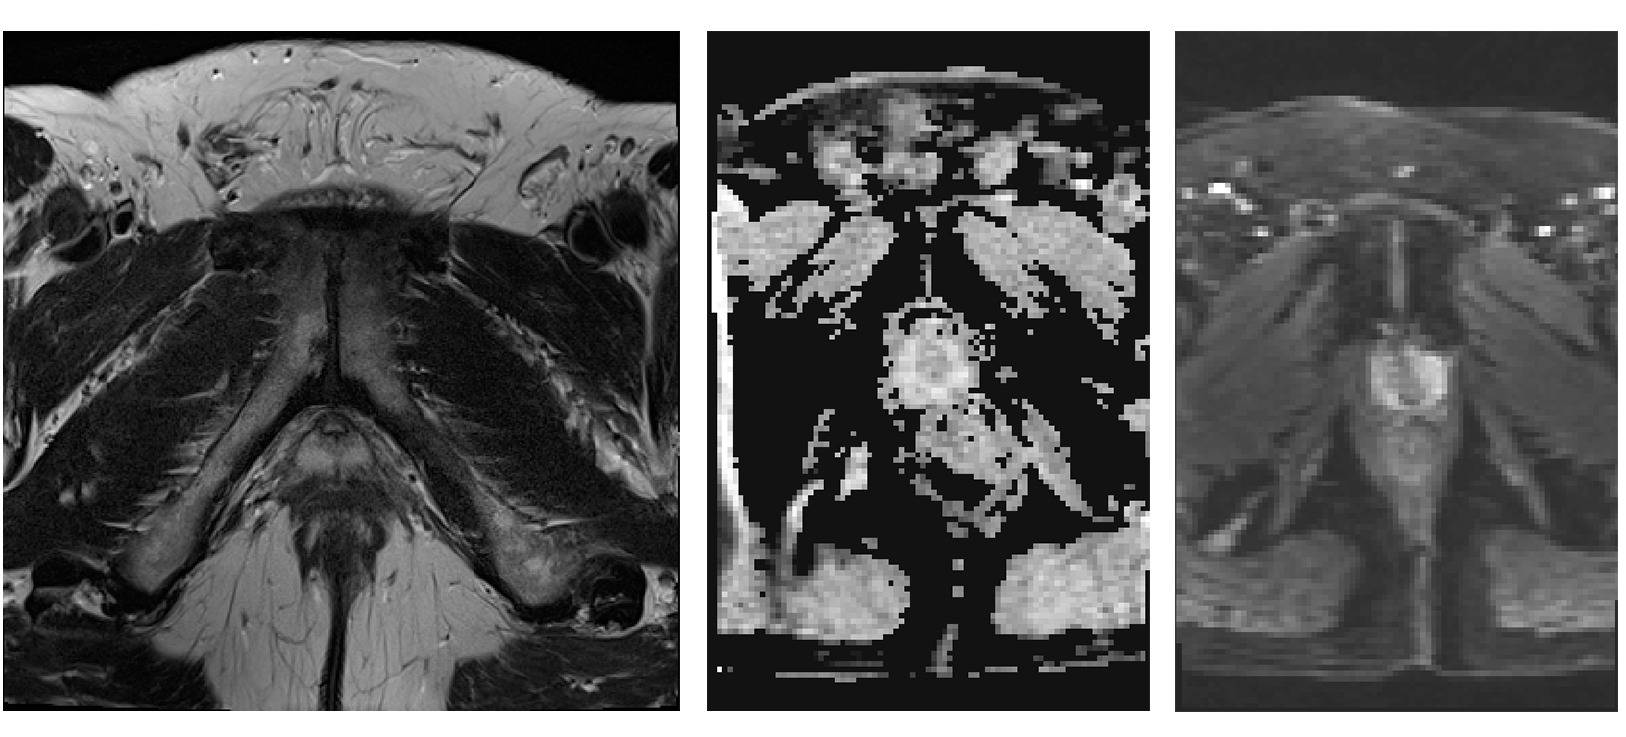
\includegraphics[width=1\textwidth, keepaspectratio=true]{./figures/PROSTATEx-t2-adc-dwi.png}
\caption{MRI - PROSTATEx - From left to right: T2-weighted, ADC and DWI}
\label{fig:PROSTATEx-t2-adc-dwi}
\end{figure}